\documentclass[main.tex]{subfiles}

\begin{document}

\subsection{Secondo esercizio}

\begin{figure}[htb]
\centering
\resizebox{.5\textwidth}{!}{\providecommand{\main}{../../..}
\documentclass[\main/main.tex]{subfiles}
\begin{document}

\subsection{Esercizio 1}

Si definisca brevemente il concetto di impatto in un problema decisionale complesso, specificando che ruolo svolga nel processo decisionale.

Si descrivano alcune possibili rappresentazioni degli impatti di un problema finito (cioè con un numero finito, e piuttosto piccolo, di alternative).

Che cosa si intende dicendo che due impatti sono indifferenti? E incomparabili?

\subsection{Soluzione esercizio 1}
Gli impatti descrivono tutto ciò che è rilevante ai fine della decisione. Essi vengono modellati matematicamente tramite la \textbf{funzione impatto} $f: X \times \Omega \rightarrow F$, dove $F$ è l'insieme degli impatti possibili, $\Omega$ quello degli esiti possibili ed $X$ quello delle decisioni possibili.

Le componenti $f_l$ di una funzione impatto $f$ vengono chiamate \textbf{indicatori} e definiscono un aspetto dell'impatto.

Nel caso \textbf{finito} gli impatti possono essere rappresentati tramite la \textbf{matrice di valutazione}, le cui righe sono le \textit{configurazioni} $(x,\omega)$ mentre le colonne sono gli \textit{indicatori} $f_l$ ed in ogni cella vi è il valore dell'indicatore per quella configurazione.

In alternativa è possibile utilizzare la \textbf{rosa dei venti} (\ref{rosa_dei_venti}), un grafico bidimensionale:

\begin{figure}
  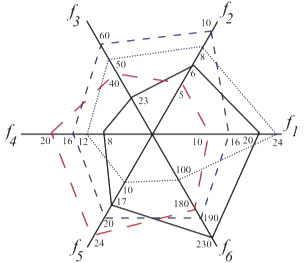
\includegraphics[width=0.5\textwidth]{rosa}
  \caption{Rosa dei venti}
  \label{rosa_dei_venti}
\end{figure}

Due impatti sono \textbf{indifferenti} quando il decisore accetta di scambiarli in entrambi i versi: $f_1 \preceq f_2  \land f_2 \preceq f_1 \Rightarrow f_1 \approx f_2$.

Due impatti sono \textbf{incomparabili} quando il decisore non accetta di scambiarli in alcun verso: $f_1 \npreceq f_2  \land f_2 \npreceq f_1 \Rightarrow f_1 \bowtie f_2$.

\end{document}}
\caption{Isostatica con biella, incastro e cerniera con forza puntiforme}
\end{figure}

L'esercizio richiede di calcolare:
\begin{enumerate}
  \item Le reazioni vincolari a terra (in A) e nel punto C;
  \item Le azioni interne nell’asta AC.
\end{enumerate}

\subsection{Soluzione secondo esercizio}
\subsubsection{Osservazioni}
Prima di iniziare l'esercizio, è importante osservare che:
\begin{itemize}
  \item La struttura forma un triangolo equilatero.
  \item Possiede un unico punto A, che la vincola a terra.
  \item L'asta BD si comporta come una \textit{biella} o \textit{pendolo semplice}.
  \item Nella struttura son presenti $2$ corpi rigidi.
  \item Nella struttura son presenti 3 vincoli, una biella, una cerniera ed un incastro.
\end{itemize}
\subsubsection{Verifica preliminare di isostaticità}
Noi sappiamo risolvere solamente sistemi isostatici, per cui verifichiamo la condizione di isostaticità: $gdv_{totali} = gdl_{totali}$
\begin{gather*}
gdl_{totali}= 3 + 3 = 6
\end{gather*}
Ci aspettiamo quindi che i gradi di vincolo siano pari a $6$:
\begin{gather*}
gdv_{totali}= gdv_{biella} + gdv_{cerniera} + gdv_{incastro}
\end{gather*}
\subparagraph{Richiami sulle cerniere interne}
\begin{definition}[Cerniera interna]
Una cerniera è detta interna quando non è fissata a terra ed è compresa tra un numero $n$ di aste tale per cui:
\[ n>1 \]
\end{definition}
\begin{theorem}[Formula delle cerniere interne]
Una cerniera interna compresa tra $n$ aste impone un numero di gradi di vincolo pari a:
\[ gdv_{cerniera} = 2(n-1) \]
\end{theorem}

Per cui, sommando i gradi di vincolo di biella, cerniera ed incastro si ottiene:
\begin{gather*}
gdv_{totali}= 1 + 2(2-1) + 3 = 6
\end{gather*}

Quindi, in base all'analisi preliminare, la struttura è \textit{isostatica}.

\subparagraph{Limiti dell'analisi dei vincoli} L'analisi dei vincoli dà un risultato decisamente limitato: esistono infatti casi in cui la struttura risulta persino \textit{iperstatica} che in base ad un'analisi dei gradi di libertà risulterebbe \textit{labile}, cioè in grado di muoversi, e strutture che questa analisi descriverebbe \textit{iperstatiche} che in realtà son \textit{labili}.
Per vedere esempi di questi casi particolari, leggete la parte relativa alla statica nell'introduzione della dispensa.

In questo corso tuttavia, solo strutture \textit{isostatiche} son considerate, per cui non preoccupiamoci oltre.

\subsubsection{Primo punto}

\begin{figure}[htb]
\centering
\resizebox{.5\textwidth}{!}{\providecommand{\main}{../../..}
\documentclass[\main/main.tex]{subfiles}
\begin{document}

\subsection{Esercizio 2}
Dato il problema di programmazione matematica

\begin{align*}
	\min f(x) & =x^2_2+x_1-4x_2                 \\
	g_1(x)    & =x^2_1+x^2_2-6x_1-4x_2+9 \leq 0 \\
	g_2(x)    & =x_2-2\leq0
\end{align*}

\begin{enumerate}[a)]
	\item Si rappresenti il problema graficamente.
	\item Si scrivano le condizioni di Karush-Kuhn-Tucker.
	\item Si determinino i punti candidati, e in particolare quello/i di minimo.
\end{enumerate}

\subsection{Soluzione esercizio 2}

a) La funzione nel suo dominio di definizione è la seguente:

\begin{figure}
	\begin{subfigure}{0.45\textwidth}
		\dddgraph{x_2}{x_1}{0}{2}{1}{5}{-3}{y^2 + x^2 -6*y - 4*x + 9 <  0 && x < 2}{x^2 + y - 4*x}
		\caption{La funzione $f(x)$}
	\end{subfigure}
	~
	\begin{subfigure}{0.45\textwidth}
		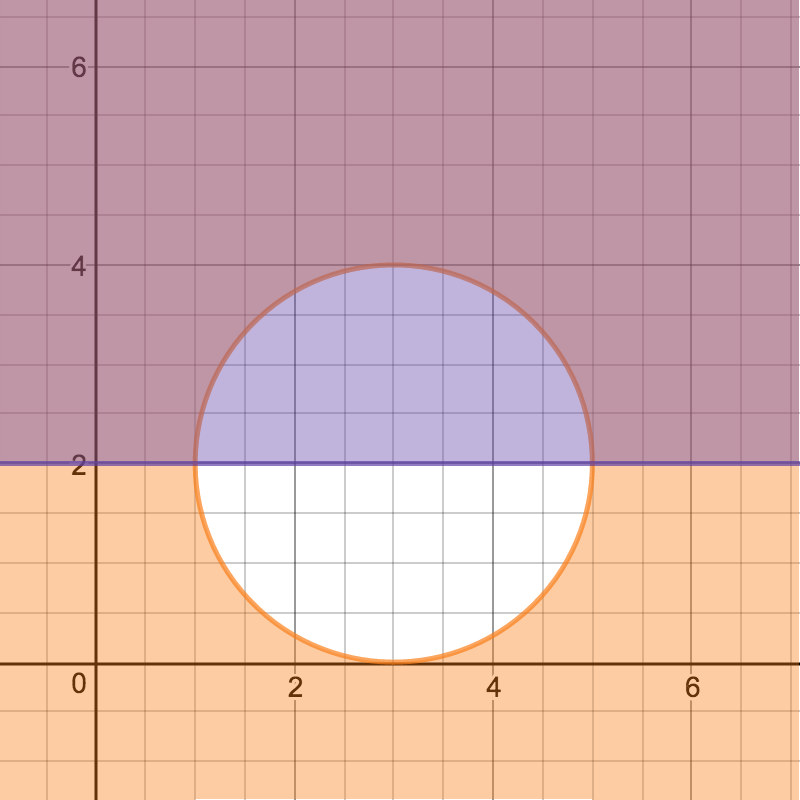
\includegraphics[width=0.8\textwidth]{10022016domain}
		\caption{Dominio della funzione $f(x)$}
	\end{subfigure}
	\caption{La funzione nel suo dominio di definizione}
\end{figure}

b) Le condizioni di Karush-Kuhn-Tucker sono le seguenti:

\begin{theorem}[Condizioni di Karush-Kuhn-Tucker]
	Sia $f$ una funzione, $h_i \text{ con } i \in \{1, \ldots, s\}$ dei vincoli bilateri e $g_j \text{ con } j \in \{1, \ldots, m\}$ dei vincoli monolateri e sia l'insieme $X$ definito come:

	\[
		X  = \{x \in \mathbb{R}^n: g_j(x) \leq 0, h_i(x) = 0 \quad \forall i, j \} \quad \text{e} \quad f, g_j, h_i \in C^1(X) \quad \forall i,j
	\]

	Se $x^*$ è un punto regolare in $X$ e un punto di minimo locale per $f \in X$, allora esistono $s$ moltiplicatori $\lambda_i \in \mathbb{R}$ e $m$ $\mu_j \geq 0$ tali che:

	\begin{align*}
		\nabla f(x^*) + \sum_{i=1}^s \lambda_i \nabla h_i(x^*) + \sum_{j=1}^m \mu_j \nabla g_j(x^*) & = 0 \\
		\mu_j g_j(x^*)                                                                              & = 0
	\end{align*}
\end{theorem}

c) Calcolo dei punti candidati.

\paragraph*{Calcolo dei punti non regolari}
I punti regolari sono quei punti nei quali i gradienti dei vincoli attivi sono fra loro linearmente indipendenti. Punti interni alle regioni di ammissibilità sono tutti regolari. Vanno investigati i punti che annullano il gradiente.

Calcolo quindi i gradienti dei due vincoli, $\nabla g_1(x)$ e $\nabla g_2(x)$:

\[
	\nabla g_1(x) = \begin{bmatrix}
		2x_1 -6 \\
		2x_2 -4
	\end{bmatrix}
	\qquad
	\nabla g_2(x) = \begin{bmatrix}
		0 \\
		1
	\end{bmatrix}
\]

Il primo gradiente si annulla per $P = (x_1 = 3, x_2 = 2)$, che è posto dove si attiva il vincolo $g_2$ ma non $g_1$ ed il secondo gradiente non si annulla mai (menchemeno in $P$) per cui $P$ è considerato regolare.

Identifichiamo ora i punti di intersezione dei vincoli:

\[
	\begin{cases}
		x^2_1+x^2_2-6x_1-4x_2+9  =  0 \\
		x_2-2 = 0
	\end{cases}
	\Rightarrow
	\begin{cases}
		x^2_1+4-6x_1-8+9  =  0 \\
		x_2 = 2
	\end{cases}
	\Rightarrow
	\begin{cases}
		x^2_1-6x_1+5  =  0 \\
		x_2 = 2
	\end{cases}
	\Rightarrow
	\begin{cases}
		x_1 = 3 \pm \sqrt{9 - 5} = 3 \pm 2 \\
		x_2 = 2
	\end{cases}
\]

I punti identificati quindi sono $A = (1, 2)$ e $B = (5, 2)$.

Verifichiamo che i gradienti siano linearmente indipendenti tramite il metodo della matrice: se per uno di essi fossero dipendenti (cioè la matrice ha determinante 0) allora $A$ non sarebbe regolare e le condizioni KKT perderebbero di validità.

\[
	\det M_g(A) = \det\begin{bmatrix}\nabla g_1(A) & \nabla g_2(A)\end{bmatrix}= \det\begin{bmatrix}
		-4 & 0 \\
		0  & 1
	\end{bmatrix}
	= -4 \neq 0
\]

\[
	\det M_g(B) = \det\begin{bmatrix}\nabla g_1(B) & \nabla g_2(B)\end{bmatrix}= \det\begin{bmatrix}
		4 & 0 \\
		0 & 1
	\end{bmatrix}
	= 4
\]


I gradienti sono linearmente indipendenti sia in $A$ che in $B$, che essendo regolari non sono punti candidati.

\paragraph*{Calcolo della lagrangiana generalizzata}
La formula della lagrangiana generalizzata (figura \ref{lagrangiana_generalizzata}) assomiglia molto alle condizioni KKT ma si applica sulle primitive (non i gradienti).

\begin{figure}
	\[
		l(x) = f(x) + \sum_{i=1}^s \lambda_i h_i(x) + \sum_{j=1}^m \mu_j g_j(x)
	\]
	\caption{Formula della lagrangiana generalizzata}
	\label{lagrangiana_generalizzata}
\end{figure}

\begin{align*}
	l(x) & = f(x) + \mu_1 g_1(x) + \mu_2 g_2(x)                               \\
	     & = x^2_2+x_1-4x_2 + \mu_1 (x^2_1+x^2_2-6x_1-4x_2+9) + \mu_2 (x_2-2)
\end{align*}

\paragraph*{Costruisco il sistema delle condizioni KKT}

\[
	\begin{cases}
		\nabla l(x) = \begin{bmatrix}
			1 + \mu_1(2x_1 - 6)                   \\
			2x_2 -4 + \mu_1(2x_2 - 4) + \mu_2 x_2 \\
		\end{bmatrix}
		= \bm{0}                            \\
		\mu_1 (x^2_1+x^2_2-6x_1-4x_2+9) = 0 \\
		\mu_2 (x_2-2) = 0                   \\
		x^2_1+x^2_2-6x_1-4x_2+9 \leq 0      \\
		x_2-2 \leq 0                        \\
		\mu_1 \geq 0                        \\
		\mu_2 \geq 0
	\end{cases}
	\Rightarrow
	\begin{cases}
		\mu_1(2x_1 - 6) = -1                      \\
		2x_2 -4 + \mu_1(2x_2 - 4) + \mu_2 x_2 = 0 \\
		\mu_2 (x_2-2) = 0                         \\
		x^2_1+x^2_2-6x_1-4x_2+9 = 0               \\
		x_2 \leq 2                                \\
		\mu_1 > 0                                 \\
		\mu_2 \geq 0
	\end{cases}
\]

Notiamo che $\mu_1$ deve essere strettamente maggiore di 0, altrimenti la prima equazione $\mu_1(2x_1 - 6) = -1$ non sarebbe rispettata. Se $\mu_1 > 0$, allora $g_1 = 0$.

Impostiamo un albero di ricerca dicotomico per risolvere il sistema, dividendo tra:

\[
	\mu_j = 0 \land g_j \leq 0 \quad \lor \quad \mu_j > 0 \land g_j = 0 \qquad \forall j \in \{1, \ldots, m\}
\]

Iniziamo scegliendo il vincolo più semplice, nel nostro caso $g_2$:

\paragraph*{Caso in cui $\mu_2 = 0 \land g_2 \leq 0$:}
\[
	\begin{cases}
		\mu_1(2x_1 - 6) = -1          \\
		2x_2 -4 + \mu_1(2x_2 - 4) = 0 \\
		x^2_1+x^2_2-6x_1-4x_2+9 = 0   \\
		x_2 \leq 2                    \\
		\mu_1 > 0
	\end{cases}
	\Rightarrow
	\begin{cases}
		\mu_1(2x_1 - 6) = -1           \\
		\textcolor{red!90}{\mu_1 = -1} \\
		x^2_1+x^2_2-6x_1-4x_2+9 = 0    \\
		x_2 \leq 2                     \\
		\textcolor{red!90}{\mu_1 > 0}
	\end{cases}
\]

Ponendo $\mu_2 = 0 \land g_2 \leq 0$ si ottiene che $\mu_1 = -1 \land \mu_1 > 0$, per cui il sistema è impossibile. Se restringiamo il caso in analisi a $\mu_2 = 0 \land g_2 = 0$ è possibile rispettare il vincolo $\mu_1 > 0$ proseguendo così:

\[
	\begin{cases}
		\mu_1(2x_1 - 6) = -1        \\
		0 = 0                       \\
		x^2_1+x^2_2-6x_1-4x_2+9 = 0 \\
		x_2 = 2                     \\
		\mu_1 > 0
	\end{cases}
	\Rightarrow
	\begin{cases}
		\mu_1(2x_1 - 6) = -1 \\
		x^2_1+4-6x_1-8+9 = 0 \\
		x_2 = 2              \\
		\mu_1 > 0
	\end{cases}
	\Rightarrow
	\begin{cases}
		\mu_1(2x_1 - 6) = -1 \\
		x^2_1-6x_1 = -5      \\
		x_2 = 2              \\
		\mu_1 > 0
	\end{cases}
	\Rightarrow
	\begin{cases}
		\mu_1 = -\frac{1}{2x_1 - 6}               \\
		x_1 = 3 \pm \sqrt{9 + 5} = 3 \pm \sqrt{4} \\
		x_2 = 2                                   \\
		\mu_1 > 0
	\end{cases}
\]

Solamente $x_1 = 1$ è accettabile poiché $\mu_1 > 0$:

\[
	\begin{cases}
		\mu_1 = -\frac{1}{2 - 6} =  \frac{1}{4} \\
		x_1 = 1                                 \\
		x_2 = 2
	\end{cases}
\]

Ne otteniamo quindi il punto candidato coincidente con $A = (1, 2)$, con $\bm{\mu} = \begin{bmatrix}
		\frac{1}{4} \\
		0
	\end{bmatrix}$.

\paragraph*{Caso in cui $\mu_2 > 0 \land g_2 = 0$:}
\[
	\begin{cases}
		\mu_1(2x_1 - 6)  = -1                     \\
		2x_2 -4 + \mu_1(2x_2 - 4) + \mu_2 x_2 = 0 \\
		x^2_1+x^2_2-6x_1-4x_2+9 = 0               \\
		x_2 = 2                                   \\
		\mu_1 > 0                                 \\
		\mu_2 > 0
	\end{cases}
	\Rightarrow
	\begin{cases}
		\mu_1(2x_1 - 6)  = -1            \\
		4 -4 + \mu_1(4 - 4) + 2\mu_2 = 0 \\
		x^2_1+4-6x_1-8+9 = 0             \\
		x_2 = 2                          \\
		\mu_1 > 0                        \\
		\mu_2 > 0
	\end{cases}
	\Rightarrow
	\begin{cases}
		\mu_1(2x_1 - 6)  = -1        \\
		\textcolor{red!90}{\mu_2 =0} \\
		x^2_1+4-6x_1-8+9 = 0         \\
		x_2 = 2                      \\
		\mu_1 > 0                    \\
		\textcolor{red!90}{\mu_2 > 0}
	\end{cases}
\]

Ponendo $\mu_2 > 0 \land g_2 = 0$ si ottiene che $\mu_2 = 0 \land \mu_2 > 0$, per cui il sistema è impossibile. Ne segue che il caso in analisi è impossibile.

\paragraph*{Calcolo del valore dei punti candidati}
Sostituisco i punti candidati nella funzione da minimizzare ed ottengo:

\[
	\begin{cases}
		f(A) = f(1,2) =  4 + 1 - 8 = -3 \\
	\end{cases}
\]

Il punto di ottimo locale (minimo) risulta essere $A = (1, 2)$.

\end{document}}
\caption{Analisi dei vincoli esterni}
\label{vincoli_esterni_1}
\end{figure}

\subparagraph{Vincoli esterni}
Iniziamo con l'analisi dei vincoli esterni (Figura \ref{vincoli_esterni_1}), che in questo caso sono unicamente A. Consideriamo quindi l'intero sistema come un corpo rigido, rimuovendo tutti i dettagli che non ci interessano e sostituiamo all'incastro in A le rispettive reazioni vincolari.

Normalmente, un vincolo ad incastro presenta 3 reazioni vincolari: una verticale ($V_A$), una orizzontale ($H_A$) ed un momento resistente ($M_A$) che si contrappone al momento imposto dalla forza esterna.

In questo caso, però, sul corpo rigido agisce una forza orientata sul piano orizzontale, senza alcuna componente verticale, per cui il vincolo a incastro non contrappone alcuna reazione verticale.

Inoltre il vettore $\vec{r}$, che rappresenta la distanza dal punto di applicazione della forza E al punto di applicazione del vincolo A, possiede unicamente una componente orizzontale, percui la forza esterna non va ad applicare alcun momento sul corpo rigido, essendo i due vettori paralleli.

Procedendo con le leggi di equilibrio della statica otteniamo:

\[
R_A : \begin{cases}
H_A - F = 0\\
V_A = 0\\
M_A = 0
\end{cases}
\Longrightarrow \begin{cases}
H_A = F\\
V_A = 0\\
M_A = 0
\end{cases}
\]

\begin{figure}[htb]
\centering
\resizebox{.5\textwidth}{!}{\providecommand{\main}{../../..}
\documentclass[\main/main.tex]{subfiles}
\begin{document}

\subsection{Exercise 3}
The following table holds values of 5 solutions with 2 cost criteria:
\begin{table}
  \begin{tabular}{L|LLLLL}
        & a_1 & a_2 & a_3 & a_4 & a_5 \\
    \hline
    f_1 & 20  & 60  & 30  & 50  & 100 \\
    f_2 & 70  & 20  & 30  & 40  & 0
  \end{tabular}
\end{table}

\begin{enumerate}[a)]
  \item Determine if there are dominated alternatives.
  \item Determine the paretian frontier with the constraints method.
  \item Determine the supported solutions and the support for each one.
\end{enumerate}

\subsection{Exercise 3 resolution}
\subsubsection*{a) Dominated alternatives}
The solution $a_3$ dominates $a_4$.

\subsubsection*{Constraints method}
First of all we plot the points on the $f_1-f_2$ plane:

\begin{figure}
  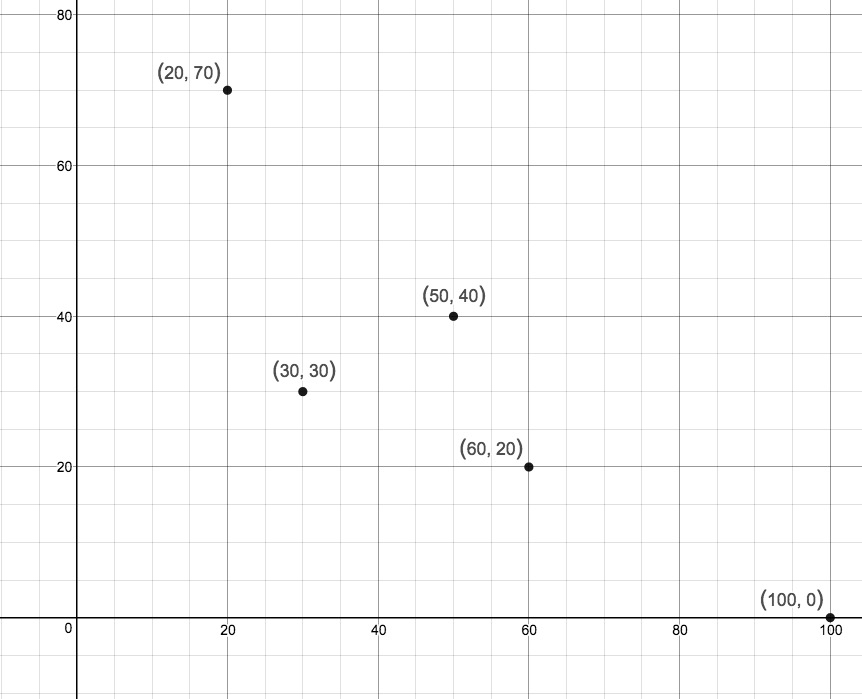
\includegraphics[width=0.4\textwidth]{20180124_03_1}
\end{figure}

Since it's a minimization problem (the indicator values are costs), the standard function will be of the kind: $f_1 \leq \epsilon$.

There are no solution for the standard $\epsilon < 20$, so it holds no interest.

\begin{figure}
  \begin{subfigure}{0.32\textwidth}
    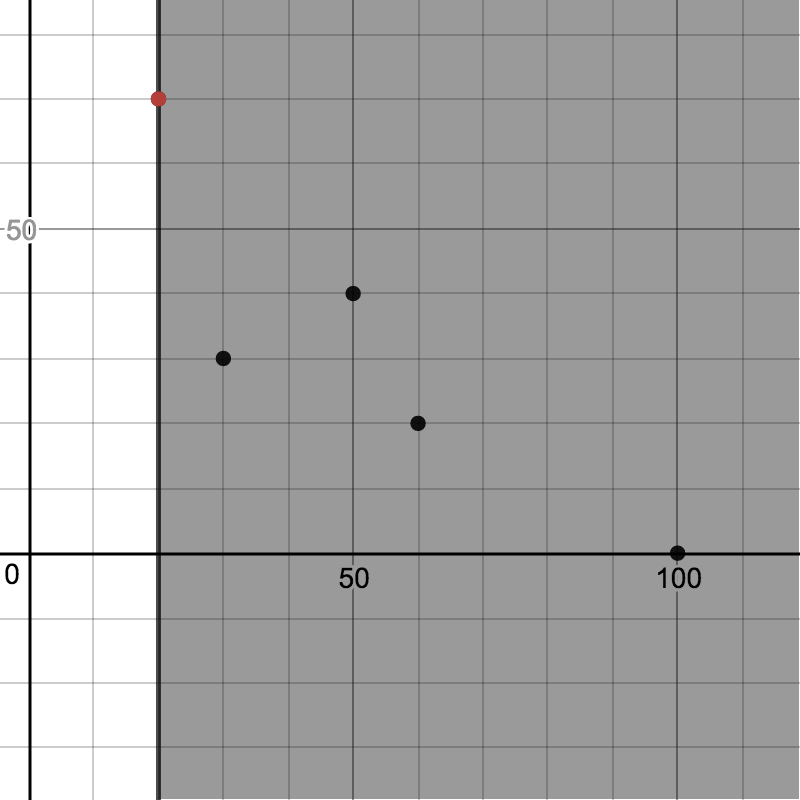
\includegraphics[width=\textwidth]{20180124_03_2}
    \caption{$\epsilon=20$, $f_1 \leq 20$, optimal solution $a_1$}
  \end{subfigure}
  \begin{subfigure}{0.32\textwidth}
    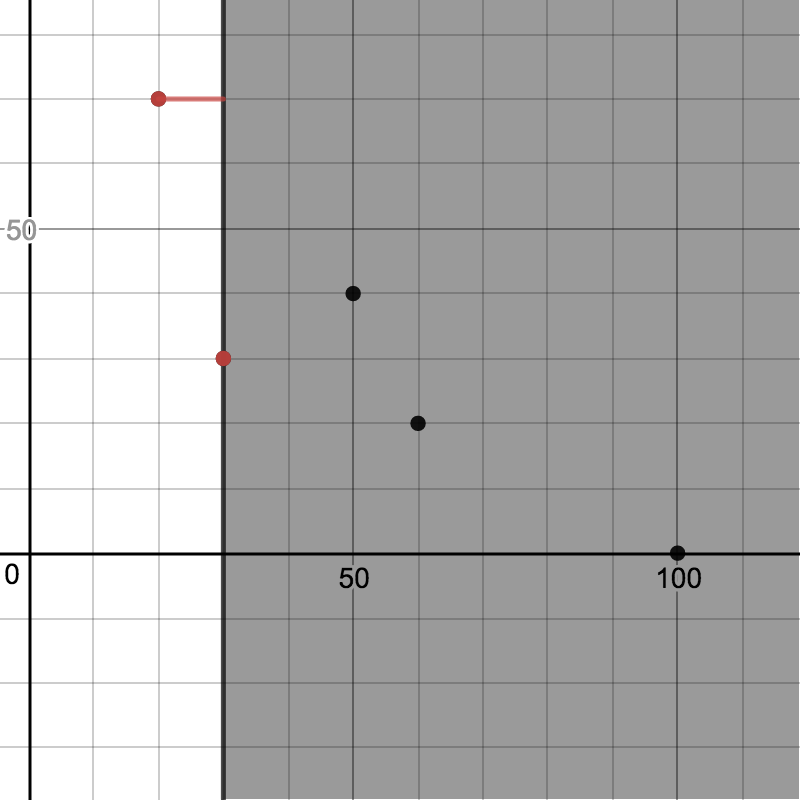
\includegraphics[width=\textwidth]{20180124_03_3}
    \caption{$\epsilon=30$, $f_1 \leq 30$, optimal solution $a_3$}
  \end{subfigure}
  \begin{subfigure}{0.32\textwidth}
    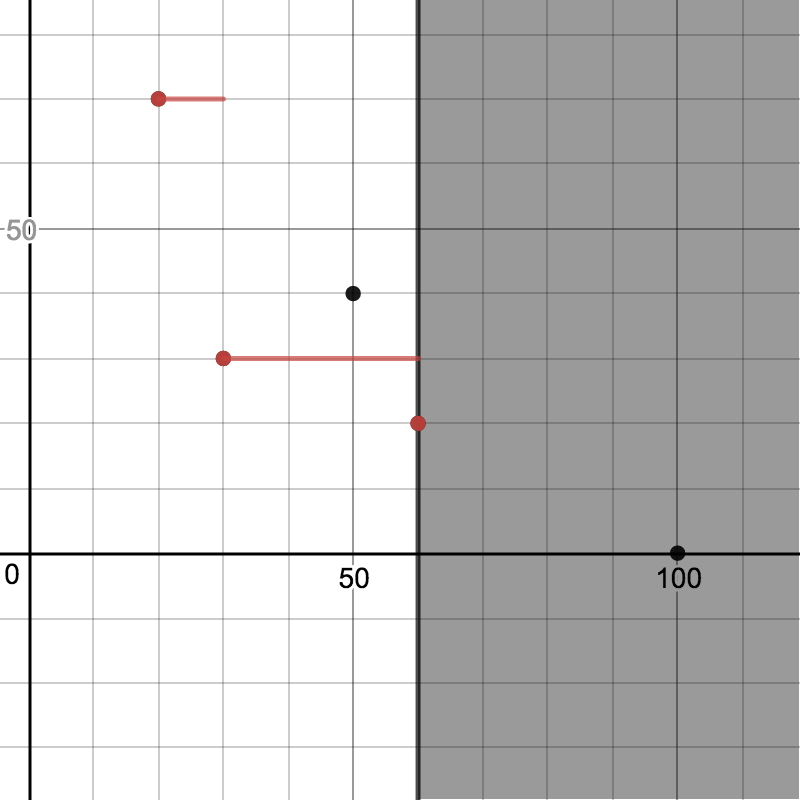
\includegraphics[width=\textwidth]{20180124_03_4}
    \caption{$\epsilon=60$, $f_1 \leq 60$, optimal solution $a_2$}
  \end{subfigure}
  \begin{subfigure}{0.32\textwidth}
    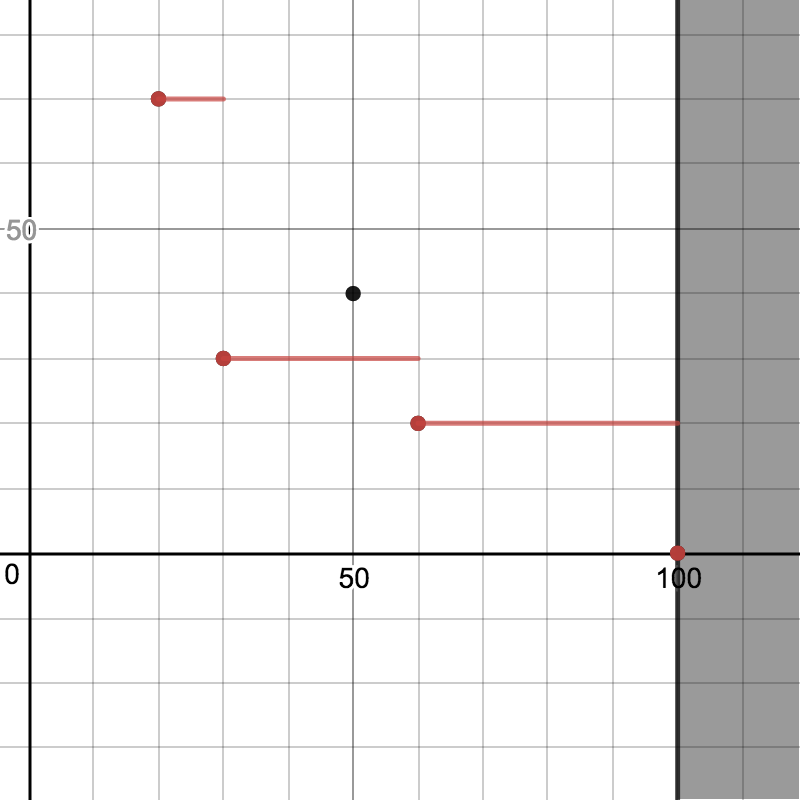
\includegraphics[width=\textwidth]{20180124_03_5}
    \caption{$\epsilon=100$, $f_1 \leq 100$, optimal solution $a_5$}
  \end{subfigure}
  \begin{subfigure}{0.32\textwidth}
    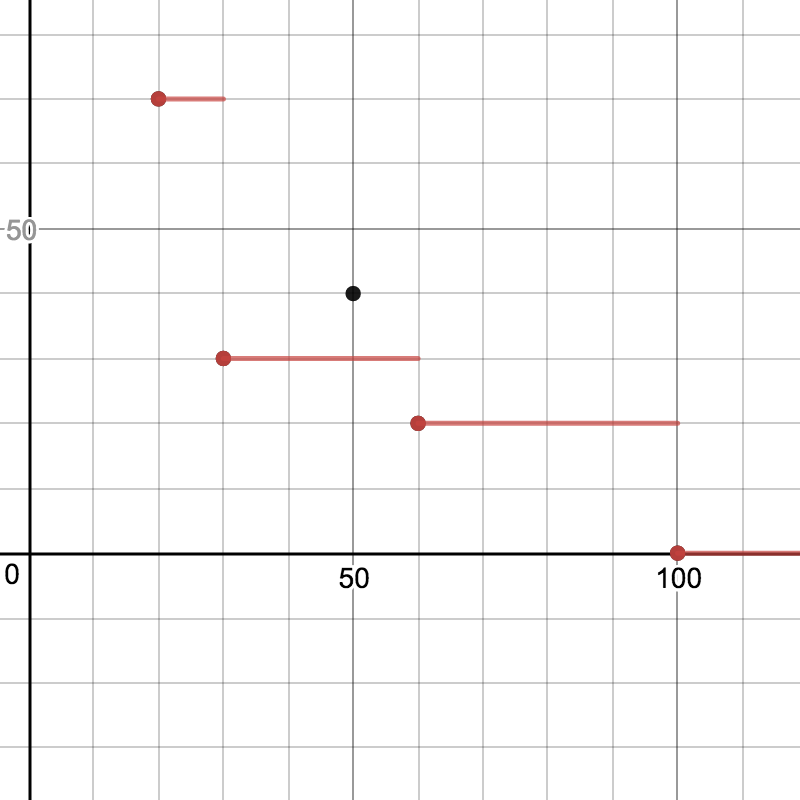
\includegraphics[width=\textwidth]{20180124_03_6}
    \caption{$\epsilon=\infty$, $f_1 \leq \infty$, optimal solution $a_5$}
  \end{subfigure}
  \caption{Paretian frontier}
\end{figure}

\subsubsection*{Solutions support}
Let's define $\w_1$ as the weight for the indicator $f_1$ and $\w_2 = 1-\w_1$ for the indicator $\w_2$.

\begin{figure}
  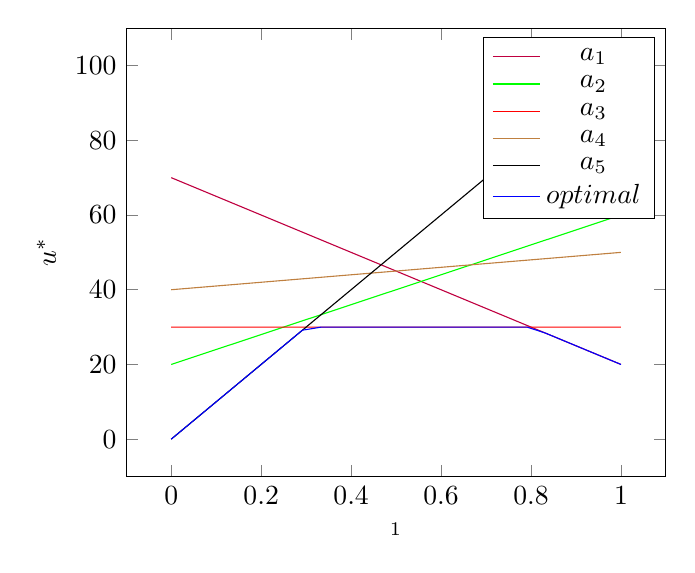
\begin{tikzpicture}
    \begin{axis}[
        xlabel=$\w_1$,
        ylabel=$u^*$,
        domain=0:1
      ]
      \addplot[mark=none,color=purple]{
        20*x+70*(1-x)
      };
      \addplot[mark=none,color=green]{
        60*x+20*(1-x)
      };
      \addplot[mark=none,color=red]{
        30*x+30*(1-x)
      };
      \addplot[mark=none,color=brown]{
        50*x+40*(1-x)
      };
      \addplot[mark=none,color=black]{
        100*x+0*(1-x)
      };
      \addplot[mark=none,color=blue]{
        min(min(min(min(
        20*x+70*(1-x),
        60*x+20*(1-x)
        ),
        30*x+30*(1-x)
        ),
        50*x+40*(1-x)
        ),
        100*x+0*(1-x)
        )
      };
      \legend{$a_1$, $a_2$, $a_3$, $a_4$, $a_5$, $optimal$}
    \end{axis}
  \end{tikzpicture}
  \caption{Supports}
\end{figure}

For $\w_1 \leq \frac{3}{10}$ the optimal solution is $a_5$.

For $\frac{3}{10} \leq \w_1 \leq \frac{4}{5}$ the optimal solution is $a_3$.

For $\w_1 \geq \frac{4}{5}$ the optimal solution is $a_1$.

\end{document}}
\caption{Analisi dell'asta CE}
\label{vincoli_asta_CE_1}
\end{figure}

\subparagraph{Asta CE}
Ora per andare a calcolare le reazioni vincolari in C, andiamo a considerare l'asta CE e ne sostituiamo i vincoli con reazioni vincolari corrispondenti (figura \ref{vincoli_asta_CE_1}).

È importante ricordare che l'asta BD agisce da biella, e una biella trasmette unicamente la reazione assiale, indirizzata appunto con l'asse della biella.

Possiamo quindi notare che nulla agisce in direzione verticale sull'asta CE, per cui la C non impone una reazione verticale.

Procediamo nuovamente con la legge dell'equilibrio della statica, scegliendo (arbitrariamente\footnote{generalmente si sceglie il punto con più forze applicate, così che non debbano essere considerate per semplificare l'equazione dell'equilibrio dei momenti. In questo caso in tutti i punti vi è applicata al più una forza, per cui è indifferente. Oltre a questo motivo, se fosse presente un momento (applicato dall'esterno, o presente per via di un momento resistente) verrebbe scelto il punto in cui vi è il momento.}) come punto in cui calcolare l'equilibrio dei momenti il punto C, otteniamo:

\[
R_C : \begin{cases}
H_C + R_D - F = 0\\
V_C = 0\\
M_C = 0 = LR_D - 2LF
\end{cases}
\Longrightarrow \begin{cases}
H_C = F - R_D\\
V_C = 0\\
R_D = 2F
\end{cases}
\Longrightarrow \begin{cases}
H_C = -F\\
V_C = 0\\
R_D = 2F
\end{cases}
\]

Siccome $\vec{H_C}$ è risultato negativo, ne abbiamo scelto una direzione "sbagliata". Poco male. Correggiamo quindi la figura, per avere un'immagine che meglio rifletta la realtà (figura \ref{vincoli_asta_CE_2}):


\begin{figure}[!tbp]
  \begin{subfigure}[b]{.5\textwidth}
  \centering
  \resizebox{.5\textwidth}{!}{ \providecommand{\main}{../../..}
\documentclass[\main/main.tex]{subfiles}

\newcommand{\defaultWrapperPrepper}[9]{
  \def\GraphArgI{#1}%
  \def\GraphArgII{#2}%
  \def\GraphArgIII{#3}%
  \def\GraphArgIV{#4}%
  \def\GraphArgV{#5}%
  \def\GraphArgVI{#6}%
  \def\GraphArgVII{#7}%
  \def\GraphArgVIII{#8}%
  \def\GraphArgIX{#9}%
  \defaultWrapperPrepperRelay
}

\newcommand{\defaultWrapperPrepperRelay}[9]{
  \def\GraphArgX{#1}%
  \def\GraphArgXI{#2}%
  \def\GraphArgXII{#3}%
  \def\GraphArgXIII{#4}%
  \def\GraphArgXIV{#5}%
  \def\GraphArgXV{#6}%
  \def\GraphArgXVI{#7}%
  \def\GraphArgXVII{#8}%
  \def\GraphArgXVIII{#9}%
  \defaultWrapperPrepperSecondRelay
}

\newcommand{\defaultWrapperPrepperSecondRelay}[9]{
  \def\GraphArgXIX{#1}%
  \def\GraphArgXX{#2}%
  \def\colorI{#3}%
  \def\colorII{#4}%
  \def\colorIII{#5}%
  \def\colorIV{#6}%
  \def\colorV{#7}%
  \def\colorVI{#8}%
  \def\colorVII{#9}%
  \defaultGraph
}

\def\red{red}
\def\blue{blue}
\def\black{black}

\NewDocumentCommand{\defaultGraph}{m m m m}{
  \def\colorVIII{#1}%
  \def\colorIX{#2}%
  \def\colorX{#3}%
  \def\defaultCuts{#4}%

  \FPsub{\substrI}{\GraphArgI}{\GraphArgXI}
  \FPsub{\substrII}{\GraphArgII}{\GraphArgXII}
  \FPsub{\substrIII}{\GraphArgIII}{\GraphArgXIII}
  \FPsub{\substrIV}{\GraphArgIV}{\GraphArgXIV}
  \FPsub{\substrV}{\GraphArgV}{\GraphArgXV}
  \FPsub{\substrVI}{\GraphArgVI}{\GraphArgXVI}
  \FPsub{\substrVII}{\GraphArgVII}{\GraphArgXVII}
  \FPsub{\substrVIII}{\GraphArgVIII}{\GraphArgXVIII}
  \FPsub{\substrIX}{\GraphArgIX}{\GraphArgXIX}
  \FPsub{\substrX}{\GraphArgX}{\GraphArgXX}


  \FPclip{\substrI}{\substrI}
  \FPclip{\substrII}{\substrII}
  \FPclip{\substrIII}{\substrIII}
  \FPclip{\substrIV}{\substrIV}
  \FPclip{\substrV}{\substrV}
  \FPclip{\substrVI}{\substrVI}
  \FPclip{\substrVII}{\substrVII}
  \FPclip{\substrVIII}{\substrVIII}
  \FPclip{\substrIX}{\substrIX}
  \FPclip{\substrX}{\substrX}

  \tikzexternaldisable
  \begin{tikzpicture}
    \tikzset{
      vertex/.style={circle,draw,minimum size=2em},
      edge/.style={->,> = latex}
    }

    % vertices
    \node[vertex] (s) at (0,2) {$s$};
    \node[vertex] (t) at (8,2) {$t$};
    \node[vertex] (1) at (2,4) {$1$};
    \node[vertex] (2) at (6,4) {$2$};
    \node[vertex] (3) at (2,0) {$3$};
    \node[vertex] (4) at (6,0) {$4$};

    %edges
    \FPifeq\GraphArgXI\zero
    \draw[edge,\colorI] (s) to node[midway, left] {\substrI}(1);
    \else
    \FPifgt\substrI\zero
    \draw[edge,\colorI] (s) to [bend right=20] node[midway, left] {\substrI}(1);
    \fi

    \FPifeq\substrI\zero
    \draw[edge,\colorI] (1) to node[midway, right] {\GraphArgXI}(s);
    \else
    \FPifgt\GraphArgXI\zero
    \draw[edge,\colorI] (1) to [bend right=20] node[midway, right] {\GraphArgXI}(s);
    \fi

    \FPifeq\substrII\zero
    \draw[edge,\colorII] (3) to node[midway, left] {\GraphArgXII}(s);
    \else
    \FPifgt\GraphArgXII\zero
    \draw[edge,\colorII] (3) to [bend right=20] node[midway, left] {\GraphArgXII}(s);
    \fi

    \FPifeq\GraphArgXII\zero
    \draw[edge,\colorII] (s) to node[midway, right] {\substrII}(3);
    \else
    \FPifgt\substrII\zero
    \draw[edge,\colorII] (s) to [bend right=20] node[midway, right] {\substrII}(3);
    \fi

    \FPifeq\GraphArgXIII\zero
    \draw[edge,\colorIII] (3) to node[midway, left] {\substrIII}(1);
    \else
    \FPifgt\substrIII\zero
    \draw[edge,\colorIII] (3) to [bend right=20] node[midway, left] {\substrIII}(1);
    \fi

    \FPifeq\substrIII\zero
    \draw[edge,\colorIII] (1) to node[midway, right] {\GraphArgXIII}(3);
    \else
    \FPifgt\GraphArgXIII\zero
    \draw[edge,\colorIII] (1) to [bend right=20] node[midway, right] {\GraphArgXIII}(3);
    \fi

    \FPifeq\GraphArgXIV\zero
    \draw[edge,\colorIV] (3) to node[midway, above] {\substrIV}(4);
    \else
    \FPifgt\substrIV\zero
    \draw[edge,\colorIV] (3) to [bend right=20] node[midway, above] {\substrIV}(4);
    \fi

    \FPifeq\substrIV\zero
    \draw[edge,\colorIV] (4) to node[midway, below] {\GraphArgXIV}(3);
    \else
    \FPifgt\GraphArgXIV\zero
    \draw[edge,\colorIV] (4) to [bend right=20] node[midway, below] {\GraphArgXIV}(3);
    \fi

    \FPifeq\GraphArgXV\zero
    \draw[edge,\colorV] (4) to node[pos=.3, left] {\substrV}(1);
    \else
    \FPifgt\substrV\zero
    \draw[edge,\colorV] (4) to [bend right=20] node[pos=.3, left] {\substrV}(1);
    \fi

    \FPifeq\substrV\zero
    \draw[edge,\colorV] (1) to node[pos=.3, right] {\GraphArgXV}(4);
    \else
    \FPifgt\GraphArgXV\zero
    \draw[edge,\colorV] (1) to [bend right=20] node[pos=.3, right] {\GraphArgXV}(4);
    \fi

    \FPifeq\GraphArgXVI\zero
    \draw[edge,\colorVI] (4) to node[midway, left] {\substrVI}(2);
    \else
    \FPifgt\substrVI\zero
    \draw[edge,\colorVI] (4) to [bend right=20] node[midway, left] {\substrVI}(2);
    \fi

    \FPifeq\substrVI\zero
    \draw[edge,\colorVI] (2) to node[midway, right] {\GraphArgXVI}(4);
    \else
    \FPifgt\GraphArgXVI\zero
    \draw[edge,\colorVI] (2) to [bend right=20] node[midway, right] {\GraphArgXVI}(4);
    \fi

    \FPifeq\GraphArgXVII\zero
    \draw[edge,\colorVII] (4) to node[midway, left] {\substrVII}(t);
    \else
    \FPifgt\substrVII\zero
    \draw[edge,\colorVII] (4) to [bend right=20] node[midway, left] {\substrVII}(t);
    \fi

    \FPifeq\substrVII\zero
    \draw[edge,\colorVII] (t) to node[midway, right] {\GraphArgXVII}(4);
    \else
    \FPifgt\GraphArgXVII\zero
    \draw[edge,\colorVII] (t) to [bend right=20] node[midway, right] {\GraphArgXVII}(4);
    \fi

    \FPifeq\GraphArgXVIII\zero
    \draw[edge,\colorVIII] (1) to node[midway, above] {\substrVIII}(2);
    \else
    \FPifgt\substrVIII\zero
    \draw[edge,\colorVIII] (1) to [bend right=20] node[midway, above] {\substrVIII}(2);
    \fi

    \FPifeq\substrVIII\zero
    \draw[edge,\colorVIII] (2) to node[midway, below] {\GraphArgXVIII}(1);
    \else
    \FPifgt\GraphArgXVIII\zero
    \draw[edge,\colorVIII] (2) to [bend right=20] node[midway, below] {\GraphArgXVIII}(1);
    \fi

    \FPifeq\GraphArgXIX\zero
    \draw[edge,\colorIX] (2) to node[midway, right] {\substrIX}(t);
    \else
    \FPifgt\substrIX\zero
    \draw[edge,\colorIX] (2) to [bend right=20] node[midway, right] {\substrIX}(t);
    \fi

    \FPifeq\substrIX\zero
    \draw[edge,\colorIX] (t) to node[midway, left] {\GraphArgXIX}(2);
    \else
    \FPifgt\GraphArgXIX\zero
    \draw[edge,\colorIX] (t) to [bend right=20] node[midway, left] {\GraphArgXIX}(2);
    \fi

    \FPifeq\GraphArgXX\zero
    \draw[edge,\colorX] (2) to node[pos=.3, right] {\substrX}(3);
    \else
    \FPifgt\substrX\zero
    \draw[edge,\colorX] (2) to [bend right=20] node[pos=.3, right] {\substrX}(3);
    \fi

    \FPifeq\substrX\zero
    \draw[edge,\colorX] (3) to node[pos=.3, left] {\GraphArgXX}(2);
    \else
    \FPifgt\GraphArgXX\zero
    \draw[edge,\colorX] (3) to [bend right=20] node[pos=.3, left] {\GraphArgXX}(2);
    \fi
    \defaultCuts
  \end{tikzpicture}
  \tikzexternalenable
}

\newcommand{\currentGraphPreloader}[9]{
  \def\currentGraphArgI{#1}%
  \def\currentGraphArgII{#2}%
  \def\currentGraphArgIII{#3}%
  \def\currentGraphArgIV{#4}%
  \def\currentGraphArgV{#5}%
  \def\currentGraphArgVI{#6}%
  \def\currentGraphArgVII{#7}%
  \def\currentGraphArgVIII{#8}%
  \def\currentGraphArgIX{#9}%
  \secondCurrentGraphPreloader
}
\newcommand{\secondCurrentGraphPreloader}[9]{
  \def\currentGraphArgX{#1}%
  \def\currentColorI{#2}%
  \def\currentColorII{#3}%
  \def\currentColorIII{#4}%
  \def\currentColorIV{#5}%
  \def\currentColorV{#6}%
  \def\currentColorVI{#7}%
  \def\currentColorVII{#8}%
  \def\currentColorVIII{#9}%
  \currentGraph
}

\NewDocumentCommand{\currentGraph}{m m O{}}{
  \def\currentColorIX{#1}%
  \def\currentColorX{#2}%
  \defaultWrapperPrepper{25}{25}{10}{25}{5}{10}{30}{35}{20}{15}{\currentGraphArgI}{\currentGraphArgII}{\currentGraphArgIII}{\currentGraphArgIV}{\currentGraphArgV}{\currentGraphArgVI}{\currentGraphArgVII}{\currentGraphArgVIII}{\currentGraphArgIX}{\currentGraphArgX}{\currentColorI}{\currentColorII}{\currentColorIII}{\currentColorIV}{\currentColorV}{\currentColorVI}{\currentColorVII}{\currentColorVIII}{\currentColorIX}{\currentColorX}{#3}
}



\begin{document}
\subsection{Esercizio 4}
Si consideri la rete sottostante in cui i valori sugli archi rappresentano le loro capacità:

\begin{figure}
  \currentGraphPreloader
  {0}{0}{0}{0}{0}
  {0}{0}{0}{0}{0}
  {\black}{\black}{\black}{\black}{\black}
  {\black}{\black}{\black}{\black}{\black}
\end{figure}

\begin{enumerate}[a)]
  \item Determinare il flusso massimo da \textbf{s} e \textbf{t} inviando nelle prime due iterazioni 5 unità lungo i percorsi $s,3,4,2,t$ e $s,3,4,1,2,t$.
  \item Riportare i cammini aumentanti ed il corrispondente aumento di flusso.
  \item SI riporti sulla figura il valore del flusso massimo.
  \item Determinare il taglio minimo.
  \item Scegliere un insieme di archi e gli si associ un costo unitario di flusso in modo che la soluzione trovata non sia a costo minimo.
\end{enumerate}

\subsection{Soluzione esercizio 4}
\subsubsection*{Step preliminare}
Invio 5 unità lungo i due percorsi indicati.

\begin{figure}
  \begin{subfigure}{0.49\textwidth}
    \currentGraphPreloader
    {0}{5}{0}{5}{0}
    {5}{0}{0}{5}{0}
    {\black}{\red}{\black}{\red}{\black}
    {\red}{\black}{\black}{\red}{\black}
    \caption{Invio 5 unità lungo $s,3,4,2,t$}
  \end{subfigure}
  \begin{subfigure}{0.49\textwidth}
    \currentGraphPreloader
    {0}{10}{0}{10}{5}
    {5}{0}{5}{10}{0}
    {\black}{\red}{\black}{\red}{\red}
    {\black}{\black}{\red}{\red}{\black}
    \caption{Invio 5 unità lungo $s,3,4,1,2,t$}
  \end{subfigure}
  \caption{Preparazione preliminare richiesta}
\end{figure}

\subsubsection*{Procedo con algoritmo}

Dallo stato corrente, procedo come segue:

\begin{figure}
  \begin{subfigure}{0.49\textwidth}
    \currentGraphPreloader
    {0}{25}{0}{25}{5}
    {5}{15}{5}{10}{0}
    {\black}{\red}{\black}{\red}{\black}
    {\black}{\red}{\black}{\black}{\black}
    \caption{Invio 15 unità lungo $s,3,4,t$}
  \end{subfigure}
  \begin{subfigure}{0.49\textwidth}
    \currentGraphPreloader
    {5}{25}{0}{25}{0}
    {5}{20}{5}{10}{0}
    {\red}{\black}{\black}{\black}{\red}
    {\black}{\red}{\black}{\black}{\black}
    \caption{Invio 5 unità lungo $s,1,4,t$}
  \end{subfigure}
  \begin{subfigure}{0.49\textwidth}
    \currentGraphPreloader
    {15}{25}{0}{25}{0}
    {5}{20}{15}{20}{0}
    {\red}{\black}{\black}{\black}{\black}
    {\black}{\black}{\red}{\red}{\black}
    \caption{Invio 10 unità lungo $s,1,2,t$}
  \end{subfigure}
  \begin{subfigure}{0.49\textwidth}
    \currentGraphPreloader
    {20}{25}{0}{25}{0}
    {10}{25}{20}{20}{0}
    {\red}{\black}{\black}{\black}{\black}
    {\red}{\red}{\red}{\black}{\black}
    \caption{Invio 5 unità lungo $s,1,2,4,t$}
  \end{subfigure}
  \caption{Procedo con algoritmo}
\end{figure}

\subsubsection*{Flusso massimo}
Il flusso massimo è di 45 unità.

\subsubsection*{Taglio minimo}
Il taglio minimo è di 45 unità. I due gruppi che divide sono $(A,t)$ e $(s,1,2,3)$

\begin{figure}
  \currentGraphPreloader
  {20}{25}{0}{25}{0}
  {10}{25}{20}{20}{0}
  {\black}{\black}{\black}{\black}{\black}
  {\black}{\black}{\black}{\black}{\black}[
  \draw[dashed,\red]
  ([yshift=10pt]$ (3)!0.7!(4) $ ) --
  ([yshift=-10pt]$ (3)!0.7!(4) $ );
  \draw[dashed,\red,rotate=-45]
  ([yshift=10pt]$ (2)!0.7!(t) $ ) --
  ([yshift=-10pt]$ (2)!0.7!(t) $ );
  ]
  \caption{Taglio minimo}
\end{figure}

\subsubsection*{Soluzione non a costo minimo}
È sufficiente scegliere costi in modo tale da creare un ciclo a costo negativo, per esempio assegnando come costi $s\rightarrow3: 1000$, $s\rightarrow1: 1$, $3\rightarrow1: 1$.

\end{document}}
  \caption{Asta CE con reazioni vincolari.}
  \end{subfigure}
  \hfill
  \begin{subfigure}[b]{.5\textwidth}
  \centering
  \resizebox{.5\textwidth}{!}{\providecommand{\main}{../../..}
\documentclass[\main/main.tex]{subfiles}
\begin{document}

\subsection{Esercizio 6}
Si consideri un problema di teoria delle decisioni con 3 soluzioni alternative, indicate da $x_1$, $x_2$ e $x_3$ e 2 stati di natura, indicati da $\omega_1$ e $\omega_2$.

Le seguenti tabelle riportano la funzione $f(x, \omega)$ che rappresenta dei benefici e le probabilità congiunte $p(\omega, y)$ degli stati di natura e dei risultati di un esperimento che può avere 2 esiti, indicati da $y_1$ e $y_2$. Qual è la strategia ottima?

\begin{figure}
  \begin{subfigure}{0.49\textwidth}
    \begin{table}
      \begin{tabular}{|L|L|L|}
        \hline
        f(x, \omega) & \omega_1 & \omega_2 \\
        \hline
        x_1          & 40       & 40       \\
        \hline
        x_2          & 100      & 0        \\
        \hline
        x_3          & 10       & 80       \\
        \hline
      \end{tabular}
    \end{table}
  \end{subfigure}
  \begin{subfigure}{0.49\textwidth}
    \begin{table}
      \begin{tabular}{|L|L|L|}
        \hline
        p(\omega, y) & \omega_1 & \omega_2 \\
        \hline
        y_1          & 0.1      & 0.4      \\
        \hline
        y_2          & 0.3      & 0.2      \\
        \hline
      \end{tabular}
    \end{table}
  \end{subfigure}
\end{figure}

\subsection{Soluzione esercizio 6}
\begin{figure}
  \begin{tikzpicture}
    \Tree[.root
    [.\text{faccio esperimento}
    [.$0.5$
      [.$y_1$
          [.$x_1$
              [.$0.2$
                  [.$\w_1$
                      [.$40$ ]
                    ]
                ]
                [.$0.8$
                  [.$\w_2$
                      [.$40$ ]
                    ]
                ]
            ]
            [.$x_2$
              [.$0.2$
                  [.$\w_1$
                      [.$100$ ]
                    ]
                ]
                [.$0.8$
                  [.$\w_2$
                      [.$0$ ]
                    ]
                ]
            ]
            [.$x_3$
              [.$0.2$
                  [.$\w_1$
                      [.$10$ ]
                    ]
                ]
                [.$0.8$
                  [.$\w_2$
                      [.$80$ ]
                    ]
                ]
            ]
        ]
    ]
    [.$0.5$
      [.$y_2$
          [.$x_1$
              [.$0.6$
                  [.$\w_1$
                      [.$40$ ]
                    ]
                ]
                [.$0.4$
                  [.$\w_2$
                      [.$40$ ]
                    ]
                ]
            ]
            [.$x_2$
              [.$0.6$
                  [.$\w_1$
                      [.$100$ ]
                    ]
                ]
                [.$0.4$
                  [.$\w_2$
                      [.$0$ ]
                    ]
                ]
            ]
            [.$x_3$
              [.$0.6$
                  [.$\w_1$
                      [.$10$ ]
                    ]
                ]
                [.$0.4$
                  [.$\w_2$
                      [.$80$ ]
                    ]
                ]
            ]
        ]
    ]
    ]
    [.\text{non faccio esperimento}
    [.$x_1$
      [.$0.4$
          [.$\w_1$
              [.$40$ ]
            ]
        ]
        [.$0.6$
          [.$\w_2$
              [.$40$ ]
            ]
        ]
    ]
    [.$x_2$
      [.$0.4$
          [.$\w_1$
              [.$100$ ]
            ]
        ]
        [.$0.6$
          [.$\w_2$
              [.$0$ ]
            ]
        ]
    ]
    [.$x_3$
      [.$0.4$
          [.$\w_1$
              [.$10$ ]
            ]
        ]
        [.$0.6$
          [.$\w_2$
              [.$80$ ]
            ]
        ]
    ]
    ]
    ]
  \end{tikzpicture}
\end{figure}

\begin{figure}
  \begin{tikzpicture}
    \Tree[.root
    [.\text{faccio esperimento}
    [.$0.5$
      [.$y_1$
          [.$x_1$
              [.$40$ ]
            ]
            [.$x_2$
              [.$20$ ]
            ]
            [.$x_3$
              [.$66$ ]
            ]
        ]
    ]
    [.$0.5$
      [.$y_2$
          [.$x_1$
              [.$40$ ]
            ]
            [.$x_2$
              [.$60$ ]
            ]
            [.$x_3$
              [.$38$ ]
            ]
        ]
    ]
    ]
    [.\text{non faccio esperimento}
    [.$x_1$
      [.$40$ ]
    ]
    [.$x_2$
      [.$40$ ]
    ]
    [.$x_3$
      [.$52$ ]
    ]
    ]
    ]
  \end{tikzpicture}
\end{figure}

Svolgendo l'esperimento ottengo un'informazione di utilità pari a $66+60-52*2 = 22$, pertanto è vantaggioso eseguirlo.

Nel caso di esito $y_1$ procedo con la scelta $x_3$ e nel caso $y_2$ procedo con $x_2$.

\end{document}
}
  \caption{Asta CE con modulo della forza esterna.}
  \end{subfigure}
  \caption{Analisi corretta dell'asta CE.}
  \label{vincoli_asta_CE_2}
\end{figure}
\subparagraph{Ricapitolo primo punto}

\[
R_A : \begin{cases}
H_A = F\\
V_A = 0\\
M_A = 0
\end{cases}
;
R_C : \begin{cases}
H_C = F\\
V_C = 0\\
M_C = 0
\end{cases}
\]

\begin{figure}[!tbp]
  \begin{subfigure}[b]{.5\textwidth}
  \centering
  \resizebox{.5\textwidth}{!}{\providecommand{\main}{../../..}
\documentclass[\main/main.tex]{subfiles}
\begin{document}

\subsection{Esercizio 5}
Viene dato il seguente problema di programmazione in condizioni di incertezza, i cui valori indicano utilità:

\begin{table}
  \begin{tabular}{|L|L|L|L|L|}
    \hline
    u_{\omega a} & a_1 & a_2 & a_3 & a_4 \\
    \hline
    \omega_1     & 50  & 40  & 60  & 90  \\
    \hline
    \omega_2     & 10  & 30  & 20  & 0   \\
    \hline
  \end{tabular}
\end{table}

\begin{enumerate}[a)]
  \item Si indichi se vi sono alternative dominate e quali alternative le dominano.
  \item Si indichi l’alternativa scelta con il criterio del caso pessimo.
  \item Si mostri come cambia l’alternativa scelta con il criterio del caso medio al variare della probabilità $\pi(\omega_1)$ del primo scenario.
\end{enumerate}

\subsection{Soluzione esercizio 5}
\subsubsection*{Alternative dominate}
Un'alternativa domina un'altra quando, senza applicare particolari criteri, questa è migliore per almeno uno degli scenari ed uguale in tutti gli altri. Cerchiamo la soluzione che dia scenari a valore massimo poichè i valori rappresentano utilità.

In questo caso, l'alternativa solamente $a_3 \prec a_1$, mentre non è possibile affermare nulla delle altre che sono preferibili l'una alle altre per almeno uno scenario.

\subsubsection*{Criterio del caso pessimo}
Nel criterio del caso pessimo, si assume che qualsiasi scelta venga effettuata accadrà il suo corrispondente caso pessimo. La scelta con scenario pessimo migliore è $a_2$.

\begin{table}
  \begin{tabular}{|L|L|L|L|L|}
    \hline
    u_{\omega a} & a_1                   & a_2                   & a_3                   & a_4                 \\
    \hline
    \omega_1     & 50                    & 40                    & 60                    & 90                  \\
    \hline
    \omega_2     & \cellcolor{red!50} 10 & \cellcolor{red!50} 30 & \cellcolor{red!50} 20 & \cellcolor{red!50}0 \\
    \hline
  \end{tabular}
  \caption{Casi pessimi in rosso}
\end{table}

\subsubsection*{Caso medio}
Il caso medio (suppongo sia, dato che non appare nelle dispense) il caso di Hurwicz con coefficiente della combinazione convessa pari $\pi(\omega_1)$ per il primo scenario (che coincide sempre con il caso ottimo) e $1-\pi(\omega_1)$ per il secondo (che coincide sempre con il caso pessimo).

\begin{table}
  \begin{tabular}{|L|L|L|L|L|}
    \hline
        & a_1                                   & a_2                                   & a_3                                   & a_4             \\
    \hline
    u_H & 50\pi(\omega_1) + 10(1-\pi(\omega_1)) & 40\pi(\omega_1) + 30(1-\pi(\omega_1)) & 60\pi(\omega_1) + 20(1-\pi(\omega_1)) & 90\pi(\omega_1) \\
    \hline
  \end{tabular}
\end{table}

\begin{figure}
  \begin{subfigure}{0.31\textwidth}
    \begin{table}[H]
      \begin{tabular}{|L|L|L|L|L|}
        \hline
            & a_1 & a_2 & a_3 & a_4 \\
        \hline
        u_H & 50  & 40  & 60  & 90  \\
        \hline
      \end{tabular}
      \caption{Caso $\pi(\omega_1)=1$: viene scelta $a_4$}
    \end{table}
  \end{subfigure}
  \begin{subfigure}{0.31\textwidth}
    \begin{table}[H]
      \begin{tabular}{|L|L|L|L|L|}
        \hline
            & a_1 & a_2 & a_3 & a_4 \\
        \hline
        u_H & 10  & 30  & 20  & 0   \\
        \hline
      \end{tabular}
      \caption{Caso $\pi(\omega_1)=0$: scelta $a_2$}
    \end{table}
  \end{subfigure}
  \begin{subfigure}{0.31\textwidth}
    \begin{tikzpicture}
      \begin{axis}[
          width= \textwidth,
          xlabel=$f$,
          ylabel=$u_H$,
          domain=0:1,
          ytick = {0,10,...,90},
          legend style={at={(0,1)},anchor=north west}
        ]
        \addplot[mark=none,color=red]{50*x + 10*(1-x)};
        \addplot[mark=none,color=blue]{40*x + 30*(1-x)};
        \addplot[mark=none,color=green]{60*x + 20*(1-x)};
        \addplot[mark=none]{90*x};
        \legend{$a_1$,$a_2$,$a_3$,$a_4$}
      \end{axis}
    \end{tikzpicture}
    \caption{L'utilità $u_H$ al variare della probabilità}
  \end{subfigure}
\end{figure}



\end{document}
}
  \caption{Reazioni vincolari nell'asta AC.}
  \end{subfigure}
  \hfill
  \begin{subfigure}[b]{.5\textwidth}
  \centering
  \resizebox{.5\textwidth}{!}{\providecommand{\main}{../../..}
\documentclass[\main/main.tex]{subfiles}
\begin{document}

\subsection{Esercizio 7}
Dato il seguente gioco a due persone:

\begin{table}
  \begin{tabular}{|L|L|L|}
    \hline
      & A     & B      \\
    \hline
    A & (0,5) & (-1,3) \\
    \hline
    B & (0,0) & (-1,3) \\
    \hline
  \end{tabular}
\end{table}

\begin{enumerate}
  \item Determinare se vi siano strategie dominate.
  \item Determinare gli eventuali punti di equilibrio (o dimostrare che non ve ne sono).
  \item Applicare il criterio del caso pessimo al gioco in forma estesa, assumendo che i due giocatori non muovano simultaneamente, ma muova prima $G_r$ e poi $G_c$.
  \item Applicare il criterio del caso pessimo al gioco in forma estesa, assumendo che i due giocatori non muovano simultaneamente, ma muova prima $G_c$ e poi $G_r$.
\end{enumerate}

\subsection{Soluzione esercizio 7}

\subsubsection*{Strategie dominate}
Non esistono strategie dominate.

\subsubsection*{Punti di equilibrio}
L'unico punto di equilibrio è per la strategia $(A,A)$.
\begin{table}
  \begin{tabular}{|L|L|L|}
    \hline
      & A                     & B              \\
    \hline
    A & (\tilde{0},\tilde{5}) & (-1,\tilde{3}) \\
    \hline
    B & (\tilde{0},0)         & (-1,\tilde{3}) \\
    \hline
  \end{tabular}
\end{table}

\subsubsection*{Criterio del caso pessimo}
Nel criterio del caso pessimo un giocatore assume che l'altro cercherà di danneggiarlo il più possibile.
\paragraph*{Prima $G_r$, poi $G_c$}
Per $G_r$ scegliere $A$ o $B$ non porta ad payoff differenti.

\paragraph*{Prima $G_c$, poi $G_r$}
$G_c$ sceglierà $B$, poichè, nel caso pessimo, $G_r$ può scegliere $B$ e imporgli un payoff pari a $0$, mentre scegliendo $B$ il payoff sarà sempre $3$.
\end{document}
}
  \caption{Asta AC con modulo della forza esterna.}
  \end{subfigure}
  \caption{Analisi dell'asta AC.}
  \label{vincoli_asta_AC_1}
\end{figure}

\subsubsection{Secondo punto}
Per calcolare le azioni interne dell'asta AC, iniziamo disegnando le reazioni vincolari (e le forze e momenti applicati, se vi fossero) che la caratterizzano (figura \ref{vincoli_asta_AC_1}). Riassumendo, sull'asta AC agiscono:

In B agisce la reazione assiale $\vec{R_D} = \vec{R_B}$ (pari ed opposta a quanto vista nell'asta CE in D);

In C agisce la reazione vincolare $\vec{H_C}$;

In A agisce la reazione vincolare $\vec{H_A}$;

\subfile{nota_componenti_vettore.tex}

\paragraph{Divisione in componenti}
Separiamo ora le singole componenti in taglio e sforzo normale.

\begin{figure}[htb]
\centering
\resizebox{.5\textwidth}{!}{% First image 2015 06 29

\begin{tikzpicture}

  \tiny

  \point{a}{0}{0};
  \point{b}{0.7}{0.866};
  \point{c}{1}{2*0.866};
  \point{g}{-1}{0};
  \point{f}{1.5}{0.866};
  \point{d}{0}{2*0.866};

  \beam{2}{a}{c};

  \load{1}{a}[240][0.5];
  \load{1}{a}[150][0.866];

  \load{1}{c}[240][0.5][-0.6];
  \load{1}{c}[150][0.866];

  \load{1}{b}[60][0.5];
  \load{1}{b}[-30][0.866][-0.1];

  % \notation{1}{a}{A}[above left];
  % \notation{1}{b}{B}[above left];
  % \notation{1}{c}{C}[above right];

\end{tikzpicture}}
\caption{Componenti nell'asta AC}
\label{separated_components_1}
\end{figure}

\subparagraph{Calcolo dello sforzo normale}
Procediamo al calcolo della componente di sforzo normale di ogni forza applicata all'asta AC:
\[
	N: \begin{cases}
		\vec{N_A} = H_A\cos(\frac{\pi}{3})\\
		\vec{N_B} = R_B\cos(-\frac{\pi}{3})\\
		\vec{N_C} = H_C\cos(\frac{\pi}{3})
	\end{cases}
	\Longrightarrow
	\begin{cases}
		\vec{N_A} = \frac{1}{2}F\\
		\vec{N_B} = F\\
		\vec{N_C} = \frac{1}{2}F
	\end{cases}
\]

\subparagraph{disegniamo il grafico dello sforzo normale}
Ricordando la convenzione dello sforzo normale, \textbf{positivo} quando produce \textit{trazione} e \textbf{negativo} quando produce \textit{contrazione},  procediamo al disegno del grafico:

Mentre si disegna un grafico di questo tipo, è importante ricordare che il grafico deve risultare, quando è verticale, di un'altezza pari al vettore che agisce in quel punto. Per esempio, nel punto B il grafico ha un'altezza complessiva pari al valore di $N_B$, così come è analogamente in A ed in C.

Si può iniziare a disegnare il grafico partendo da un qualsiasi estremo del corpo rigido.

Iniziamo per esempio dall'estremo A. Spostiamoci di un $ds$ verso l'alto e osserviamo per questo \textit{concio elementare} se lo sforzo normale sia di trazione o contrazione. In questo caso, lo sforzo è di contrazione, per cui nella nostra convenzione definiamo il valore come negativo. Procedendo via via lungo l'asta, arriviamo al punto B, in cui è applicata una nuova forza. Qui, sommiamo i due valori dello sforzo e procediamo oltre. Da questo punto, siccome $N_B>N_A$ lo sforzo diviene di trazione e così rimane sino alla fine dell'asta in C.

Come già detto, se si esegue la stessa operazione partendo dall'estremo C al posto che in A si \textit{deve} ottenere lo stesso risultato.

\begin{figure}[!tbp]
  \begin{subfigure}[b]{.5\textwidth}
  \centering
  \resizebox{.5\textwidth}{!}{% First image 2015 06 29

\begin{tikzpicture}

  \tiny

  \point{a}{0}{0};
  \point{b}{0.7}{0.866};
  \point{b1}{0.5}{0.866};
  \point{c}{1}{2*0.866};
  \point{g}{-1}{0};
  \point{f}{1.5}{0.866};
  \point{d}{0}{2*0.866};

  \point{m1}{0.25}{0.5*0.866};
  \point{m2}{0.75}{1.5*0.866};

  \beam{2}{a}{c};

  \load{1}{a}[240][0.5];

  \load{1}{c}[240][0.5][-0.6];

  \load{1}{b}[60][0.5];

  % \notation{1}{a}{A}[above left];
  % \notation{1}{b}{B}[above left];
  % \notation{1}{c}{C}[above right];

\end{tikzpicture}}
  \caption{Sforzi normali baricentrici in AC.}
  \end{subfigure}
  \hfill
  \begin{subfigure}[b]{.5\textwidth}
  \centering
  \resizebox{.5\textwidth}{!}{\begin{tikzpicture}

  \tiny

  \point{a}{0}{0};
  \point{b}{0.5}{0.866};
  \point{c}{1}{2*0.866};
  \point{g}{-1}{0};
  \point{f}{1.5}{0.866};
  \point{d}{0}{2*0.866};

  \beam{2}{a}{c};

  \internalforces{a}{b}{0.5}{0.5}[0][blue];
  \internalforces{b}{c}{-0.5}{-0.5}[0][red];

\end{tikzpicture}}
  \caption{Grafico dello sforzo normale.}
  \end{subfigure}
  \caption{Analisi dello sforzo normale nell'asta AC.}
\end{figure}

\subparagraph{Calcolo del taglio}
Procediamo al calcolo della componente di taglio di ogni forza applicata all'asta AC:

\[
	T: \begin{cases}
		\vec{T_A} = H_A\sin(\frac{\pi}{3})\\
		\vec{T_B} = R_B\sin(-\frac{\pi}{3})\\
		\vec{T_C} = H_C\sin(\frac{\pi}{3})
	\end{cases}
	\Longrightarrow
	\begin{cases}
		\vec{T_A} = \frac{\sqrt{3}}{2}F\\
		\vec{T_B} = -\sqrt{3}F\\
		\vec{T_C} = \frac{\sqrt{3}}{2}F
	\end{cases}
\]

\subparagraph{disegniamo il grafico del taglio}
Ricordando la convenzione del taglio, \textbf{positivo} quando produce \textit{rotazione oraria} e \textbf{negativo} quando produce \textit{rotazione anti-oraria},  procediamo al disegno del grafico:

Mentre si disegna un grafico di questo tipo, è importante ricordare che il grafico deve risultare, quando è verticale, di un'altezza pari al vettore che agisce in quel punto. Per esempio, nel punto B il grafico ha un'altezza complessiva pari al valore di $T_B$, così come è analogamente in A ed in C.

Si può iniziare a disegnare il grafico partendo da un qualsiasi estremo del corpo rigido.

Iniziamo per esempio dall'estremo A. Spostiamoci di un $ds$ verso l'alto e osserviamo per questo \textit{concio elementare} se il taglio produca rotazione oraria o anti-oraria. In questo caso, produce una rotazione anti-oraria. Procedendo via via lungo l'asta, arriviamo al punto B, in cui è applicata una nuova forza. Qui, sommiamo i due valori del taglio e procediamo oltre. Da questo punto, siccome $T_B>T_A$ il taglio produce una rotazione oraria e così rimane sino alla fine dell'asta in C.

Come già detto, se si esegue la stessa operazione partendo dall'estremo C al posto che in A si \textit{deve} ottenere lo stesso risultato.

\begin{figure}[!tbp]
  \begin{subfigure}[b]{.5\textwidth}
  \centering
  \resizebox{.5\textwidth}{!}{% First image 2015 06 29

\begin{tikzpicture}

  \tiny

  \point{a}{0}{0};
  \point{b}{0.7}{0.866};
  \point{c}{1}{2*0.866};
  \point{g}{-1}{0};
  \point{f}{1.5}{0.866};
  \point{d}{0}{2*0.866};

  \beam{2}{a}{c};

  \load{1}{a}[150][0.866];

  \load{1}{c}[150][0.866];

  \load{1}{b}[-30][0.866][-0.1];

  % \notation{1}{a}{A}[above left];
  % \notation{1}{b}{B}[above left];
  % \notation{1}{c}{C}[above right];

\end{tikzpicture}}
  \caption{Taglio in AC.}
  \end{subfigure}
  \hfill
  \begin{subfigure}[b]{.5\textwidth}
  \centering
  \resizebox{.5\textwidth}{!}{% First image 2015 06 29

\begin{tikzpicture}

  \tiny

  \point{a}{0}{0};
  \point{b}{0.5}{0.866};
  \point{c}{1}{2*0.866};
  \point{g}{-1}{0};
  \point{f}{1.5}{0.866};
  \point{d}{0}{2*0.866};

  \beam{2}{a}{c};

  \internalforces{a}{b}{0.866}{0.866}[0][blue];
  \internalforces{b}{c}{-0.866}{-0.866}[0][red];

\end{tikzpicture}}
  \caption{Grafico del taglio.}
  \end{subfigure}
  \caption{Analisi del taglio nell'asta AC.}
\end{figure}

\subparagraph{Calcolo del momento flettente}
Procediamo al calcolo della componente del momento flettente. Scegliamo, per esempio, A come punto di origine del nostro calcolo del momento flettente. Un qualsiasi altro estremo dovrà dare lo stesso risultato.

La forza normale all'asta (che in questo caso è $T_A$) che viene applicata in A, se per un attimo immaginiamo l'asta come duttile, \textit{piega l'asta verso destra}. In A quindi, le fibre saranno \textit{tese sul lato di sinistra}.

Chiamiamo $\Delta{S}$ la distanza dal punto A. Il momento, in un generico punto tra A e B, sarà pari quindi a $M = \Delta{S}T_A$. Quando arriviamo in B, viene introdotta un'altra forza normale all'asta, $T_B$, di direzione opposta. Chiamiamo la distanza dal punto B $\Delta{k}$ e procediamo. Questo porta il momento a divenire pari a $M = \Delta{S}T_A - \Delta{K}T_B$, e gradualmente riduce il valore del momento sino ad azzerarsi in C.

Come già detto, se si esegue la stessa operazione partendo dall'estremo C al posto che in A si \textit{deve} ottenere lo stesso risultato.

\[
	M_{max} = \Delta{S}_{M_{max}}T_A = LT_A = L\frac{\sqrt{3}}{2}F
\]

\begin{figure}[!tbp]
  \begin{subfigure}[b]{.5\textwidth}
  \centering
  \resizebox{.5\textwidth}{!}{% First image 2015 06 29

\begin{tikzpicture}

  \tiny

  \point{a}{0}{0};
  \point{b}{0.7}{0.866};
  \point{c}{1}{2*0.866};
  \point{g}{-1}{0};
  \point{f}{1.5}{0.866};
  \point{d}{0}{2*0.866};

  \beam{2}{a}{c};

  \load{1}{a}[150][0.866];

  \load{1}{c}[150][0.866];

  \load{1}{b}[-30][0.866][-0.1];

  % \notation{1}{a}{A}[above left];
  % \notation{1}{b}{B}[above left];
  % \notation{1}{c}{C}[above right];

\end{tikzpicture}}
  \caption{Forze che producono momento flettente in AC.}
  \end{subfigure}
  \hfill
  \begin{subfigure}[b]{.5\textwidth}
  \centering
  \resizebox{.5\textwidth}{!}{% First image 2015 06 29

\begin{tikzpicture}

  \tiny

  \point{a}{0}{0};
  \point{b}{0.5}{0.866};
  \point{c}{1}{2*0.866};
  \point{g}{-1}{0};
  \point{f}{1.5}{0.866};
  \point{d}{0}{2*0.866};

  \beam{2}{a}{c};

  \internalforces{a}{b}{0}{-0.866}[0][red];
  \internalforces{b}{c}{-0.866}{0}[0][red];

\end{tikzpicture}}
  \caption{Grafico del momento flettente.}
  \end{subfigure}
  \caption{Analisi del momento flettente nell'asta AC.}
\end{figure}

\paragraph{Visualizzazione della sovrapposizione degli effetti}
Questo può essere un utile strumento per visualizzare l'effetto di ogni singola forza, anche se in alcune combinazioni questi effetti considerati uno per volta possono non avere una reale controparte fisica.

\subparagraph{Sovrapposizione degli effetti per lo sforzo normale}
Disegnando l'effetto di una sola forza per volta (figura \ref{sforzo_forza_singola}), l'effetto delle forze accoppiate due a due  (figura \ref{sforzo_coppia_forze}) si capisce come l'applicazione di forze diverse in punti diversi vada a imporre uno sforzo normale differente.

\begin{figure}[!tbp]
  \begin{subfigure}[b]{.3\textwidth}
  \centering
  \resizebox{.5\textwidth}{!}{\begin{tikzpicture}

  \tiny

  \point{a}{0}{0};
  \point{b}{0.5}{0.866};
  \point{c}{1}{2*0.866};
  \point{g}{-1}{0};
  \point{f}{1.5}{0.866};
  \point{d}{0}{2*0.866};

  \beam{2}{a}{c};

  \internalforces{a}{c}{0.5}{0.5}[0][blue];
  % \internalforces{b}{c}{-0.5}{-0.5}[0][red];

\end{tikzpicture}}
  \caption{Sforzo normale di $N_A$.}
  \end{subfigure}
  \hfill
  \begin{subfigure}[b]{.3\textwidth}
  \centering
  \resizebox{.5\textwidth}{!}{\begin{tikzpicture}

  \tiny

  \point{a}{0}{0};
  \point{b}{0.5}{0.866};
  \point{c}{1}{2*0.866};
  \point{g}{-1}{0};
  \point{f}{1.5}{0.866};
  \point{d}{0}{2*0.866};

  \beam{2}{a}{c};

  \internalforces{a}{b}{0.5}{0.5}[0][blue];
  \internalforces{b}{c}{-0.5}{-0.5}[0][red];

\end{tikzpicture}}
  \caption{Sforzo normale di $N_B$.}
  \end{subfigure}
  \hfill
  \begin{subfigure}[b]{.3\textwidth}
  \centering
  \resizebox{.5\textwidth}{!}{\begin{tikzpicture}

  \tiny

  \point{a}{0}{0};
  \point{b}{0.5}{0.866};
  \point{c}{1}{2*0.866};
  \point{g}{-1}{0};
  \point{f}{1.5}{0.866};
  \point{d}{0}{2*0.866};

  \beam{2}{a}{c};

  \internalforces{a}{c}{-0.5}{-0.5}[0][red];

\end{tikzpicture}}
  \caption{Sforzo normale di $N_C$.}
  \end{subfigure}
  \caption{Sforzo normale delle singole forze.}
  \label{sforzo_forza_singola}
\end{figure}

\begin{figure}[!tbp]
  \begin{subfigure}[b]{.3\textwidth}
  \centering
  \resizebox{.5\textwidth}{!}{\begin{tikzpicture}

  \tiny

  \point{a}{0}{0};
  \point{b}{0.5}{0.866};
  \point{c}{1}{2*0.866};
  \point{g}{-1}{0};
  \point{f}{1.5}{0.866};
  \point{d}{0}{2*0.866};

  \beam{2}{a}{c};

  \internalforces{a}{b}{1}{1}[0][blue];

\end{tikzpicture}}
  \caption{Sforzo normale di $N_A$ e $N_B$.}
  \end{subfigure}
  \hfill
  \begin{subfigure}[b]{.3\textwidth}
  \centering
  \resizebox{.5\textwidth}{!}{\begin{tikzpicture}

  \tiny

  \point{a}{0}{0};
  \point{b}{0.5}{0.866};
  \point{c}{1}{2*0.866};
  \point{g}{-1}{0};
  \point{f}{1.5}{0.866};
  \point{d}{0}{2*0.866};

  \beam{2}{a}{c};

  \internalforces{b}{c}{-1}{-1}[0][red];

\end{tikzpicture}}
  \caption{Sforzo normale di $N_B$ e $N_C$.}
  \end{subfigure}
  \hfill
  \begin{subfigure}[b]{.3\textwidth}
  \centering
  \resizebox{.5\textwidth}{!}{\begin{tikzpicture}

  \tiny

  \point{a}{0}{0};
  \point{b}{0.5}{0.866};
  \point{c}{1}{2*0.866};
  \point{g}{-1}{0};
  \point{f}{1.5}{0.866};
  \point{d}{0}{2*0.866};

  \beam{2}{a}{c};

\end{tikzpicture}}
  \caption{Sforzo normale di $N_C$ e $N_A$.}
  \end{subfigure}
  \caption{Sforzo normale di forze accoppiate due a due.}
  \label{sforzo_coppia_forze}
\end{figure}

\subparagraph{Sovrapposizione degli effetti per il taglio}
Disegnando l'effetto di una sola forza per volta (figura \ref{taglio_forza_singola}), l'effetto delle forze accoppiate due a due  (figura \ref{taglio_coppia_forze}) si capisce come l'applicazione di forze diverse in punti diversi vada a imporre un taglio differente.

\begin{figure}[!tbp]
  \begin{subfigure}[b]{.3\textwidth}
  \centering
  \resizebox{.5\textwidth}{!}{\begin{tikzpicture}

  \tiny

  \point{a}{0}{0};
  \point{b}{0.5}{0.866};
  \point{c}{1}{2*0.866};
  \point{g}{-1}{0};
  \point{f}{1.5}{0.866};
  \point{d}{0}{2*0.866};

  \beam{2}{a}{c};

  \internalforces{a}{c}{0.866}{0.866}[0][blue];

\end{tikzpicture}}
  \caption{Taglio di $T_A$.}
  \end{subfigure}
  \hfill
  \begin{subfigure}[b]{.3\textwidth}
  \centering
  \resizebox{.5\textwidth}{!}{\begin{tikzpicture}

  \tiny

  \point{a}{0}{0};
  \point{b}{0.5}{0.866};
  \point{c}{1}{2*0.866};
  \point{g}{-1}{0};
  \point{f}{1.5}{0.866};
  \point{d}{0}{2*0.866};

  \beam{2}{a}{c};

  \internalforces{a}{b}{0.866}{0.866}[0][blue];
  \internalforces{b}{c}{-0.866}{-0.866}[0][red];

\end{tikzpicture}}
  \caption{Taglio di $T_B$.}
  \end{subfigure}
  \hfill
  \begin{subfigure}[b]{.3\textwidth}
  \centering
  \resizebox{.5\textwidth}{!}{\begin{tikzpicture}

  \tiny

  \point{a}{0}{0};
  \point{b}{0.5}{0.866};
  \point{c}{1}{2*0.866};
  \point{g}{-1}{0};
  \point{f}{1.5}{0.866};
  \point{d}{0}{2*0.866};

  \beam{2}{a}{c};

  \internalforces{a}{c}{-0.866}{-0.866}[0][red];

\end{tikzpicture}}
  \caption{Taglio di $T_C$.}
  \end{subfigure}
  \caption{Taglio delle singole forze.}
  \label{taglio_forza_singola}
\end{figure}

\begin{figure}[!tbp]
  \begin{subfigure}[b]{.3\textwidth}
  \centering
  \resizebox{.5\textwidth}{!}{\begin{tikzpicture}

  \tiny

  \point{a}{0}{0};
  \point{b}{0.5}{0.866};
  \point{c}{1}{2*0.866};
  \point{g}{-1}{0};
  \point{f}{1.5}{0.866};
  \point{d}{0}{2*0.866};

  \beam{2}{a}{c};

  \internalforces{a}{b}{2*0.866}{2*0.866}[0][blue];

\end{tikzpicture}}
  \caption{Taglio di $T_A$ e $T_B$.}
  \end{subfigure}
  \hfill
  \begin{subfigure}[b]{.3\textwidth}
  \centering
  \resizebox{.5\textwidth}{!}{\begin{tikzpicture}

  \tiny

  \point{a}{0}{0};
  \point{b}{0.5}{0.866};
  \point{c}{1}{2*0.866};
  \point{g}{-1}{0};
  \point{f}{1.5}{0.866};
  \point{d}{0}{2*0.866};

  \beam{2}{a}{c};

  \internalforces{b}{c}{-2*0.866}{-2*0.866}[0][red];

\end{tikzpicture}}
  \caption{Taglio di $T_B$ e $T_C$.}
  \end{subfigure}
  \hfill
  \begin{subfigure}[b]{.3\textwidth}
  \centering
  \resizebox{.5\textwidth}{!}{\begin{tikzpicture}

  \tiny

  \point{a}{0}{0};
  \point{b}{0.5}{0.866};
  \point{c}{1}{2*0.866};
  \point{g}{-1}{0};
  \point{f}{1.5}{0.866};
  \point{d}{0}{2*0.866};

  \beam{2}{a}{c};

\end{tikzpicture}}
  \caption{Taglio di $T_C$ e $T_A$.}
  \end{subfigure}
  \caption{Taglio di forze accoppiate due a due.}
  \label{taglio_coppia_forze}
\end{figure}

\subparagraph{Sovrapposizione degli effetti per il momento flettente}
È possibile calcolare il momento flettente anche tramite la sovrapposizione degli effetti di tutte le varie forze che agiscono in direzione normale rispetto allo spostamento.

A seguire, disegnando l'effetto di una sola forza per volta (figura \ref{momento_forza_singola}), l'effetto delle forze accoppiate due a due  (figura \ref{momento_coppia_forze}) si capisce come l'applicazione di forze diverse in punti diversi vada a formare dei momenti flettenti diversi.

\begin{figure}[!tbp]
  \begin{subfigure}[b]{.3\textwidth}
  \centering
  \resizebox{.5\textwidth}{!}{% First image 2015 06 29

\begin{tikzpicture}

  \tiny

  \point{a}{0}{0};
  \point{b}{0.5}{0.866};
  \point{c}{1}{2*0.866};
  \point{g}{-1}{0};
  \point{f}{1.5}{0.866};
  \point{d}{0}{2*0.866};

  \beam{2}{a}{c};

  \internalforces{a}{c}{0}{-2*0.866}[0][red];

\end{tikzpicture}}
  \caption{Momento flettente di $T_A$.}
  \end{subfigure}
  \hfill
  \begin{subfigure}[b]{.3\textwidth}
  \centering
  \resizebox{.5\textwidth}{!}{% First image 2015 06 29

\begin{tikzpicture}

  \tiny

  \point{a}{0}{0};
  \point{b}{0.5}{0.866};
  \point{c}{1}{2*0.866};
  \point{g}{-1}{0};
  \point{f}{1.5}{0.866};
  \point{d}{0}{2*0.866};

  \beam{2}{a}{c};

  \internalforces{c}{a}{0}{2*0.866}[0][red];

\end{tikzpicture}}
  \caption{Momento flettente di $T_B$.}
  \end{subfigure}
  \hfill
  \begin{subfigure}[b]{.3\textwidth}
  \centering
  \resizebox{.5\textwidth}{!}{% First image 2015 06 29

\begin{tikzpicture}

  \tiny

  \point{a}{0}{0};
  \point{b}{0.5}{0.866};
  \point{c}{1}{2*0.866};
  \point{g}{-1}{0};
  \point{f}{1.5}{0.866};
  \point{d}{0}{2*0.866};

  \beam{2}{a}{c};

  \internalforces{b}{a}{0}{-2*0.866}[0][blue];
  \internalforces{b}{c}{0}{2*0.866}[0][blue];

\end{tikzpicture}}
  \caption{Momento flettente di $T_C$.}
  \end{subfigure}
  \caption{Momento flettente delle singole forze.}
  \label{momento_forza_singola}
\end{figure}

\begin{figure}[!tbp]
  \begin{subfigure}[b]{.3\textwidth}
  \centering
  \resizebox{.5\textwidth}{!}{% First image 2015 06 29

\begin{tikzpicture}

  \tiny

  \point{a}{0}{0};
  \point{b}{0.5}{0.866};
  \point{c}{1}{2*0.866};
  \point{g}{-1}{0};
  \point{f}{1.5}{0.866};
  \point{d}{0}{2*0.866};

  \beam{2}{a}{c};

  \internalforces{a}{c}{-2*0.866}{-2*0.866}[0][red];

\end{tikzpicture}}
  \caption{Momento flettente di $T_A$ e $T_B$.}
  \end{subfigure}
  \hfill
  \begin{subfigure}[b]{.3\textwidth}
  \centering
  \resizebox{.5\textwidth}{!}{% First image 2015 06 29

\begin{tikzpicture}

  \tiny

  \point{a}{0}{0};
  \point{b}{0.5}{0.866};
  \point{c}{1}{2*0.866};

  \point{m}{0.66*1}{0.66*2*0.866};

  \beam{2}{a}{c};

  \internalforces{a}{b}{0}{-0.866}[0][red];
  \internalforces{b}{m}{-0.866}{0}[0][red];
  \internalforces{m}{c}{0}{2*0.866}[0][blue];


\end{tikzpicture}}
  \caption{Momento flettente di $T_B$ e $T_C$.}
  \end{subfigure}
  \hfill
  \begin{subfigure}[b]{.3\textwidth}
  \centering
  \resizebox{.5\textwidth}{!}{% First image 2015 06 29

\begin{tikzpicture}

  \tiny

  \point{a}{0}{0};
  \point{b}{0.5}{0.866};
  \point{c}{1}{2*0.866};

  \point{m}{0.33*1}{0.33*2*0.866};

  \beam{2}{a}{c};

  \internalforces{c}{b}{0}{0.866}[0][red];
  \internalforces{b}{m}{0.866}{0}[0][red];
  \internalforces{m}{a}{0}{-2*0.866}[0][blue];


\end{tikzpicture}}
  \caption{Momento flettente di $T_C$ e $T_A$.}
  \end{subfigure}
  \caption{Momento flettente di forze accoppiate due a due.}
  \label{momento_coppia_forze}
\end{figure}

\end{document}